\documentclass[11pt,a4paper]{article}
\usepackage[dvipsnames]{xcolor}
% !TeX root = ./main.tex


%%%%%%%%%%%%%%%%%%%%%%%%%%%%%%%%%%%%%%%%%
% Lachaise Assignment
% Structure Specification File
% Version 1.0 (26/6/2018)
%
% This template originates from:
% http://www.LaTeXTemplates.com
%
% Authors:
% Marion Lachaise & François Févotte
% Vel (vel@LaTeXTemplates.com)
%
% License:
% CC BY-NC-SA 3.0 (http://creativecommons.org/licenses/by-nc-sa/3.0/)
% 
%%%%%%%%%%%%%%%%%%%%%%%%%%%%%%%%%%%%%%%%%

%----------------------------------------------------------------------------------------
%	PACKAGES AND OTHER DOCUMENT CONFIGURATIONS
%----------------------------------------------------------------------------------------

\usepackage{amsmath,amsfonts,stmaryrd,amssymb} % Math packages


\usepackage{graphicx}

\usepackage{booktabs} % Booktabs for beautiful tables 

\usepackage{tabularx} % The column(s) specified with the 'X' specifier will be stretched to make the table as wide as specified

\usepackage{enumerate} % Custom item numbers for enumerations

\usepackage[ruled]{algorithm2e} % Algorithms

\usepackage[framemethod=tikz]{mdframed} % Allows defining custom boxed/framed environments

\usepackage[skip=12pt]{caption}

\usepackage{listings} % File listings, with syntax highlighting
\lstset{
	basicstyle=\ttfamily, % Typeset listings in monospace font
}


\definecolor{MidnightRed}{RGB}{112,25,25}
\definecolor{MidnightBlue}{rgb}{0.1, 0.1, 0.44}

\usepackage{hyperref}
\hypersetup{
    colorlinks=true,
	linkcolor=MidnightRed,
	citecolor=MidnightRed,
    filecolor=MidnightRed,      
    urlcolor=MidnightBlue,
}

%----------------------------------------------------------------------------------------
%	DOCUMENT MARGINS
%----------------------------------------------------------------------------------------

\usepackage{geometry} % Required for adjusting page dimensions and margins


\geometry{
	paper=a4paper, % Paper size, change to letterpaper for US letter size
%	top=2.5cm, % Top margin
%	bottom=3cm, % Bottom margin
%	left=3.5cm, % Left margin
%	right=3.5cm, % Right margin
%	headheight=14pt, % Header height
%	footskip=1.5cm, % Space from the bottom margin to the baseline of the footer
%	headsep=1.2cm, % Space from the top margin to the baseline of the header
%	%showframe, % Uncomment to show how the type block is set on the page
}

%----------------------------------------------------------------------------------------
%	FONTS
%----------------------------------------------------------------------------------------

\usepackage[utf8]{inputenc} % Required for inputting international characters
\usepackage[T1]{fontenc} % Output font encoding for international characters

%\usepackage{XCharter} % Use the XCharter fonts

%----------------------------------------------------------------------------------------
%	COMMAND LINE ENVIRONMENT
%----------------------------------------------------------------------------------------

% Usage:
% \begin{commandline}
%	\begin{verbatim}
%		$ ls
%		
%		Applications	Desktop	...
%	\end{verbatim}
% \end{commandline}

\mdfdefinestyle{commandline}{
	leftmargin=10pt,
	rightmargin=10pt,
	innerleftmargin=15pt,
	middlelinecolor=black!50!white,
	middlelinewidth=2pt,
	frametitlerule=false,
	backgroundcolor=black!5!white,
	frametitle={Command Line},
	frametitlefont={\normalfont\sffamily\color{white}\hspace{-1em}},
	frametitlebackgroundcolor=black!50!white,
	nobreak,
}

% Define a custom environment for command-line snapshots
\newenvironment{commandline}{
	\medskip
	\begin{mdframed}[style=commandline]
}{
	\end{mdframed}
	\medskip
}

%----------------------------------------------------------------------------------------
%	FILE CONTENTS ENVIRONMENT
%----------------------------------------------------------------------------------------

% Usage:
% \begin{file}[optional filename, defaults to "File"]
%	File contents, for example, with a listings environment
% \end{file}

\mdfdefinestyle{file}{
	innertopmargin=1.6\baselineskip,
	innerbottommargin=0.8\baselineskip,
	topline=false, bottomline=false,
	leftline=false, rightline=false,
	leftmargin=2cm,
	rightmargin=2cm,
	singleextra={%
		\draw[fill=black!10!white](P)++(0,-1.2em)rectangle(P-|O);
		\node[anchor=north west]
		at(P-|O){\ttfamily\mdfilename};
		%
		\def\l{3em}
		\draw(O-|P)++(-\l,0)--++(\l,\l)--(P)--(P-|O)--(O)--cycle;
		\draw(O-|P)++(-\l,0)--++(0,\l)--++(\l,0);
	},
	nobreak,
}

% Define a custom environment for file contents
\newenvironment{file}[1][File]{ % Set the default filename to "File"
	\medskip
	\newcommand{\mdfilename}{#1}
	\begin{mdframed}[style=file]
}{
	\end{mdframed}
	\medskip
}

%----------------------------------------------------------------------------------------
%	NUMBERED QUESTIONS ENVIRONMENT
%----------------------------------------------------------------------------------------

% Usage:
% \begin{question}[optional title]
%	Question contents
% \end{question}

\mdfdefinestyle{question}{
	innertopmargin=1.2\baselineskip,
	innerbottommargin=0.8\baselineskip,
	roundcorner=5pt,
	nobreak,
	singleextra={%
		\draw(P-|O)node[xshift=1em,anchor=west,fill=white,draw,rounded corners=5pt]{%
		Question %\theQuestion%
		%\questionTitle%
		};
	},
}

\newcounter{Question} % Stores the current question number that gets iterated with each new question

% Define a custom environment for numbered questions
\newenvironment{question}[1][\unskip]{
	%\bigskip
	%\stepcounter{Question}
	\newcommand{\questionTitle}{~#1}
	\begin{mdframed}[style=question]
}{
	\end{mdframed}
	\medskip
}

%----------------------------------------------------------------------------------------
%	WARNING TEXT ENVIRONMENT
%----------------------------------------------------------------------------------------

% Usage:
% \begin{warn}[optional title, defaults to "Warning:"]
%	Contents
% \end{warn}

\mdfdefinestyle{warning}{
	topline=false, bottomline=false,
	leftline=false, rightline=false,
	nobreak,
	singleextra={%
		\draw(P-|O)++(-0.5em,0)node(tmp1){};
		\draw(P-|O)++(0.5em,0)node(tmp2){};
		\fill[black,rotate around={45:(P-|O)}](tmp1)rectangle(tmp2);
		\node at(P-|O){\color{white}\scriptsize\bf !};
		\draw[very thick](P-|O)++(0,-1em)--(O);%--(O-|P);
	}
}

% Define a custom environment for warning text
\newenvironment{warn}[1][Warning:]{ % Set the default warning to "Warning:"
	\medskip
	\begin{mdframed}[style=warning]
		\noindent{\textbf{#1}}
}{
	\end{mdframed}
}

%----------------------------------------------------------------------------------------
%	INFORMATION ENVIRONMENT
%----------------------------------------------------------------------------------------

% Usage:
% \begin{info}[optional title, defaults to "Info:"]
% 	contents
% 	\end{info}

\mdfdefinestyle{info}{%
	topline=false, bottomline=false,
	leftline=false, rightline=false,
	nobreak,
	singleextra={%
		\fill[black](P-|O)circle[radius=0.4em];
		\node at(P-|O){\color{white}\scriptsize\bf i};
		\draw[very thick](P-|O)++(0,-0.8em)--(O);%--(O-|P);
	}
}

% Define a custom environment for information
\newenvironment{info}[1][Info:]{ % Set the default title to "Info:"
	\medskip
	\begin{mdframed}[style=info]
		\noindent{\textbf{#1}}
}{
	\end{mdframed}
}


\renewcommand{\arraystretch}{1.2}


\usepackage[english]{varioref}
\usepackage[english]{babel}
\usepackage{datetime}
\usepackage{amsmath}
\usepackage{booktabs}
\usepackage{placeins}
\usepackage{url}
\usepackage{csquotes}
\usepackage{adjustbox}
\usepackage{listings}
\usepackage{float}
\usepackage{textcomp}
\usepackage{marginnote}
%\usepackage{enumitem}
\usepackage{graphicx}

\usepackage{minted}
%\usepackage[top=2.5cm, bottom=2.5cm, outer=5cm, inner=4cm, heightrounded, marginparwidth=3cm, marginparsep=0.5cm]{geometry}
%\renewcommand\raggedrightmarginnote{\sloppy}
%\renewcommand\raggedleftmarginnote{\sloppy}

\usepackage{vhistory}



\newlength{\storeparskip}
\setlength{\storeparskip}{\parskip}

\setlength{\parskip}{\baselineskip}%
\setlength{\parindent}{0pt}%


\newcommand{\currentversion}{1.9}

\setminted{
frame=lines,
framesep=2mm,
baselinestretch=1.1,
fontsize=\footnotesize,
linenos,
breaklines
}

\title{Network Capturing and Manipulation Introduction to Wireshark and Scapy}
\author{Gilles Callebaut\\ \texttt{gilles.callebaut@kuleuven.be}}
\date{Ghent Technology Campus, KU Leuven\\ \today \\ v\currentversion}



\begin{document} \sloppy


\maketitle

\vfill
{\footnotesize
This document is subjected to change, please consult the most recent version at: \url{github.com/GillesC/Network-Capturing-and-Manipulation----Introduction-to-Wireshark-and-Scapy}.
}

\clearpage

\begin{versionhistory}
    \vhEntry{1.0}{25/04/2019}{GC}{Created}
    \vhEntry{1.1}{01/04/2019}{GC}{Revised deadlines}
    \vhEntry{1.2}{29/04/2019}{GC}{Clarify Question 4 and Update Listing~\ref{listing:stealth-scanning}}
    \vhEntry{1.3}{12/03/2020}{GC}{Updated deadlines and removed Anaconda}
    \vhEntry{1.4}{15/03/2020}{GC}{Adjusted so the lab session could be done at home}
    \vhEntry{1.5}{29/03/2020}{GC}{Added example scapy project set-up Section~\ref{sec:getting-to-know-scapy}}
    \vhEntry{1.6}{18/04/2020}{GC}{Updated questions with more details and report description}
    \vhEntry{1.6.1}{20/04/2020}{GC}{Update Q8 and the report}
    \vhEntry{1.7}{08/03/2021}{GC}{Added case studies}
    \vhEntry{1.8}{16/09/2021}{GC}{Updates case studies}
    \vhEntry{\currentversion}{03/01/2022}{GC}{Moved from reports to small intermediate tests at the end of each session.}
    
\end{versionhistory}
\clearpage

\setcounter{tocdepth}{2}
\tableofcontents
\clearpage

\section{Introduction}
One's understanding of network protocols can often be greatly deepened by ``seeing
protocols in action'' and by ``playing around with protocols'' – observing the sequence of messages exchanged between two protocol entities, delving down into the details of protocol operation, and causing protocols to perform certain actions and then observing these actions and their consequences. This can be done in simulated scenarios or in a ``real'' network environment such as the Internet. 

In these labs you will be observing as well as manipulating the network protocols in your computer ``in action'' interacting and exchanging messages with protocol entities executing elsewhere in the Internet. 
You could think of a network packet analyzer as a measuring device used to examine what's going on inside a network cable, just like a voltmeter is used by an electrician to examine what's going on inside an electric cable. We will focus on Wireshark to monitor packets and Scapy, a Python library, to manipulate them. 

The first goal of this lab is to introduce you to Wireshark and get you acquainted with it's interface. The following questions will demonstrate that you have been able to get Wireshark up and running, and have explored some of its capabilities.
But first, install Wireshark and capture some data!

\section{Getting to know Wireshark}
In this first Wireshark lab, you will get acquainted with Wireshark, and make some simple packet captures and observations.
The basic tool for observing the messages exchanged between executing protocol entities is called a packet sniffer. As the name suggests, a packet sniffer captures (``sniffs'') messages being sent/received from/by your computer; it will also typically store and/or display the contents of the various protocol fields in these captured messages. A packet sniffer itself is passive. It observes messages being sent and received by applications and protocols running on your computer, but never sends packets itself. Similarly, received packets are never explicitly addressed to the packet sniffer. Instead, a packet sniffer receives a copy of packets that are sent/received from/by application and protocols executing on your machine.

\begin{question}
    Is Wireshark able to capture packets that are not addressed to your computer?
\end{question}

\subsection{Installing Wireshark}
In order to run Wireshark, you will need to have access to a computer that supports both Wireshark and the libpcap or WinPCap packet capture library. 
In case you are unable to see any interfaces when opening Wireshark, the libcap software is probably not installed. Usually, the libpcap software will be installed for you when you install Wireshark.

\begin{question}
    What is the purpose of the libcap software?
\end{question}

\subsection{Running Wireshark}
When you run the Wireshark program, you'll get a startup screen that looks something
like the screen below. Different versions of Wireshark will have different startup screens
-- so don't panic if yours doesn't look exactly like the screen below!

\begin{figure}[h]
    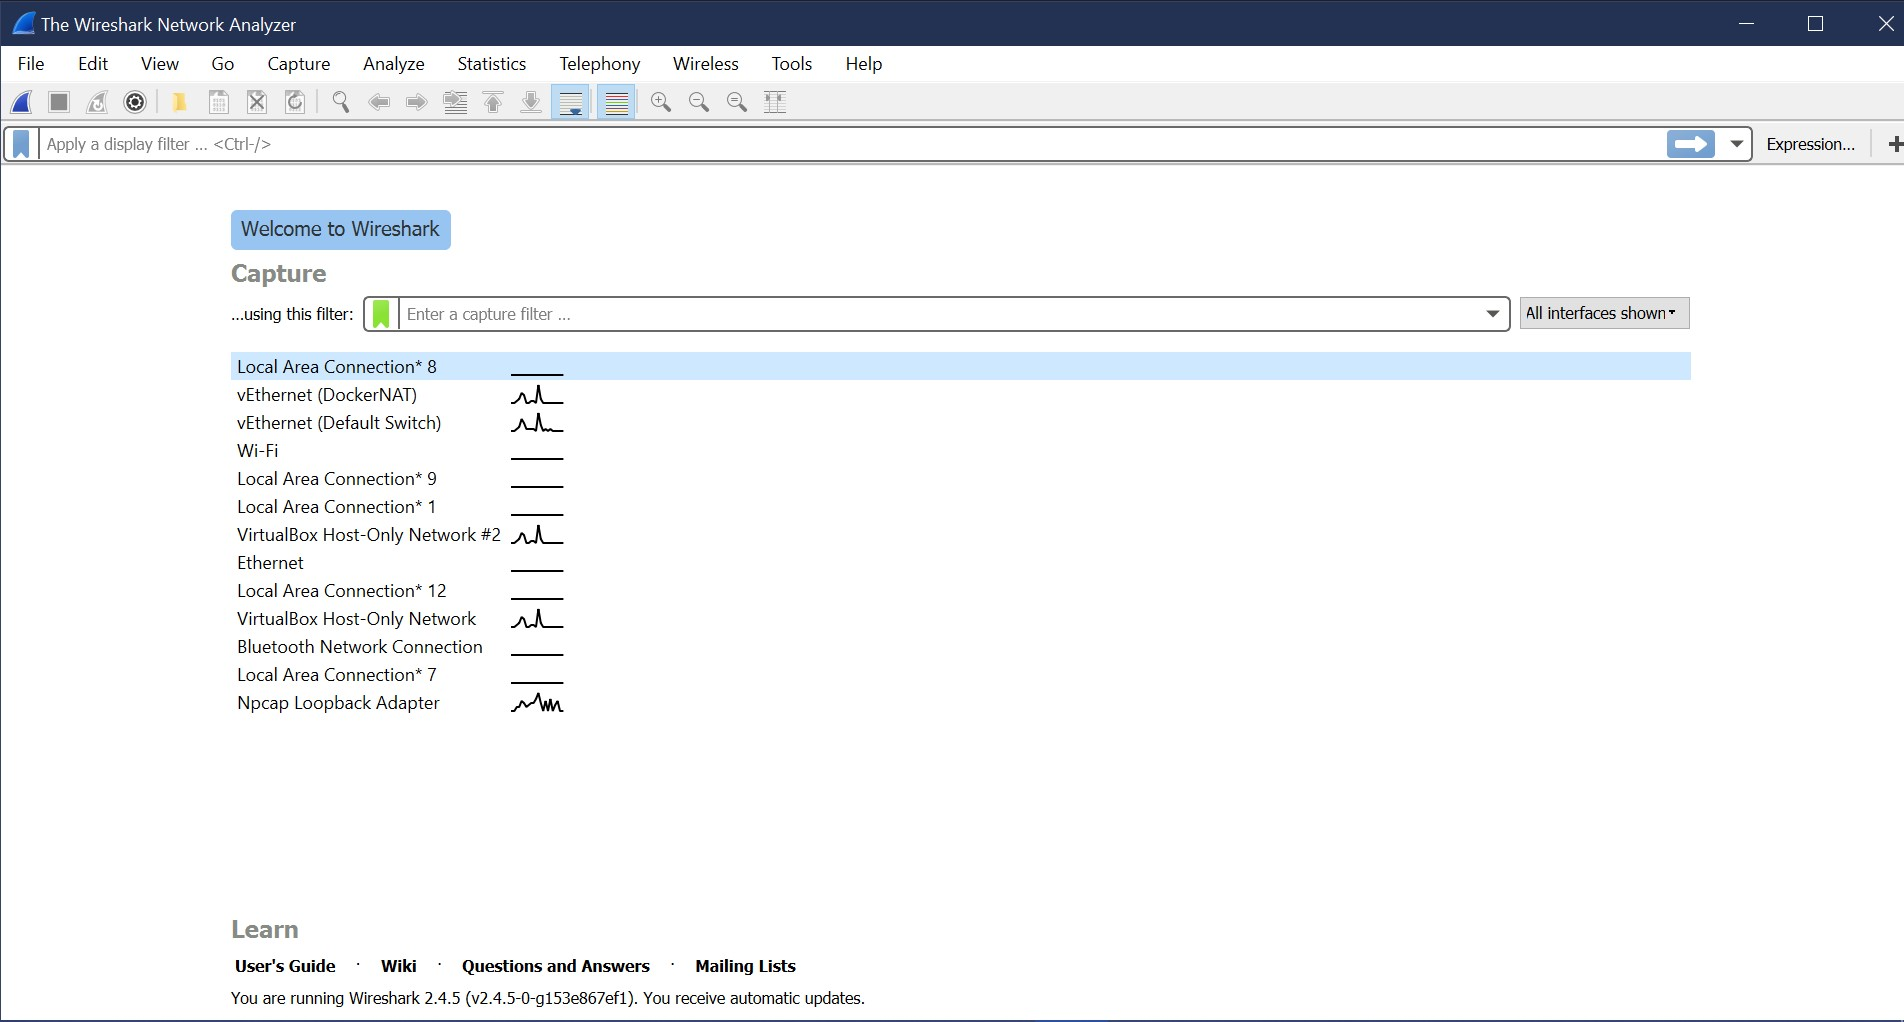
\includegraphics[width=\textwidth]{start_screen.jpg}
    \caption{Initial Wireshark Screen}\label{fig:init-screen}
\end{figure}

There's not much interesting on this screen. But note that under the Capture section,
there is a list of so-called interfaces. Be sure to locate the interface on the startup page through which you are getting Internet
connectivity, e.g., mostly likely a WiFi or Ethernet interface, and select that interface.

\begin{question}
    Try to explain the different interfaces displayed on the first screen. You can find out more about the interfaces by running \texttt{Get-NetAdapter -IncludeHidden} in Windows PowerShell.
\end{question}

Let's take Wireshark out for a spin! If you click on one of these interfaces to start packet
capture (i.e., for Wireshark to begin capturing all packets being sent to/from that
interface), a screen like the one below will be displayed, showing information about the
packets being captured. Once you start packet capture, you can stop it by using the
Capture pull down menu and selecting Stop.

\begin{figure}[H]
    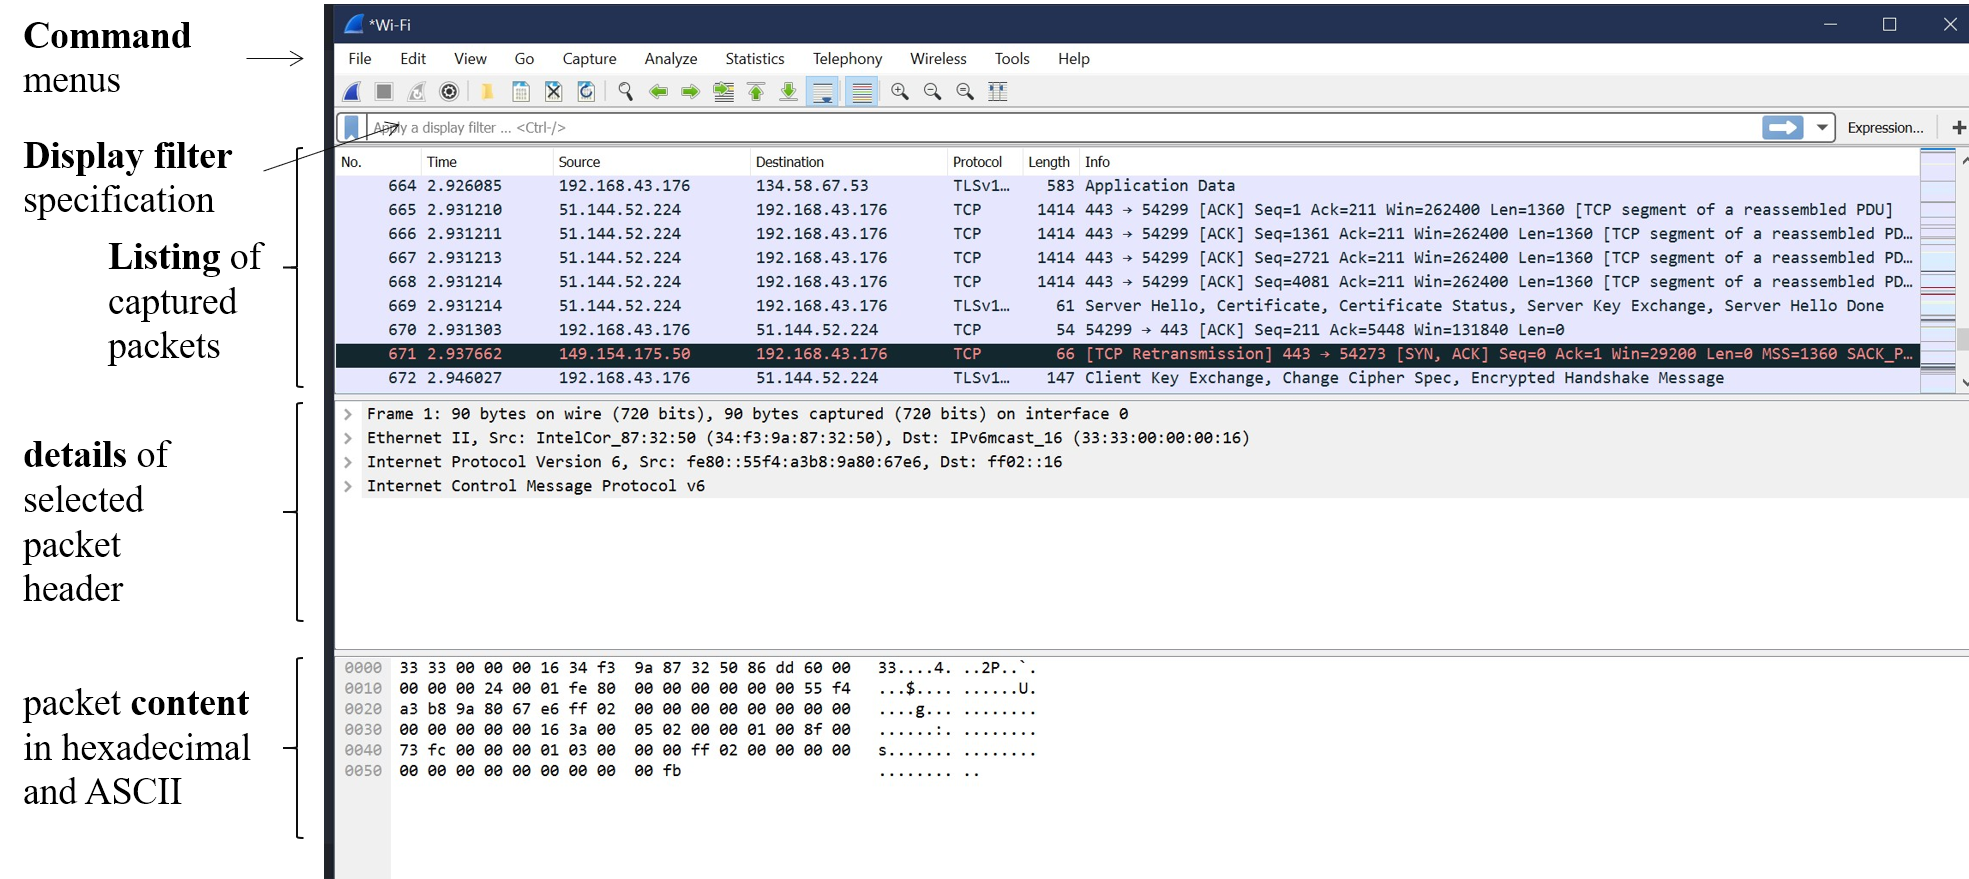
\includegraphics[width=\textwidth]{capturing.png}
    \caption{Wireshark Graphical User Interface, during packet capture and analysis.}%
    \label{fig:packet_capt}
\end{figure}

This looks more interesting! The Wireshark interface has five major components:
\begin{itemize}
    \item The \textbf{command menus} are standard pulldown menus located at the top of the
    window. Of interest to us now are the File and Capture menus. The File menu
    allows you to save captured packet data or open a file containing previously
    captured packet data, and exit the Wireshark application. The Capture menu
    allows you to begin packet capture.
    \item The \textbf{packet-listing window} displays a one-line summary for each packet captured, including the packet number (assigned by Wireshark; this is not a packet number contained in any protocol's header), the time at which the packet was captured, the packet's source and destination addresses, the protocol type,  and protocol-specific information contained in the packet. The packet listing can be sorted according to any of these categories by clicking on a column name. The protocol type field lists the highest-level protocol that sent or received this packet, i.e., the protocol that is the source or ultimate sink for this packet.
    \item The \textbf{packet-header details window} provides details about the packet selected (highlighted) in the packet-listing window. (To select a packet in the packetlisting window, place the cursor over the packet's one-line summary in the packet-listing window and click with the left mouse button.). These details include information about the Ethernet frame (assuming the packet was sent/received over an Ethernet interface) and IP datagram that contains this packet. The amount of Ethernet and IP-layer detail displayed can be expanded or minimized by clicking on the caret signs to the left of the Ethernet frame or IP datagram line in the packet details window. If the packet has been carried over TCP or UDP, TCP or UDP details will also be displayed, which can similarly be expanded or minimized. Finally, details about the highest-level protocol that sent or received this packet are also provided.
    \item The \textbf{packet-contents window} displays the entire contents of the captured frame, in both ASCII and hexadecimal format.
    \item Towards the top of the Wireshark graphical user interface, is the \textbf{packet display filter field}, into which a protocol name or other information can be entered in order to filter the information displayed in the packet-listing window (and hence the packet-header and packet-contents windows). In the example below, we'll use the packet-display filter field to have Wireshark hide (not display) packets except those that correspond to HTTP messages.
\end{itemize}

\subsection{Taking Wireshark for a Test Run}

\begin{enumerate}
    \item Start up your favorite web browser, which will display your selected homepage.
    \item Start up the Wireshark software. You will initially see a window similar to that
    shown in Figure~\ref{fig:init-screen}. Wireshark has not yet begun capturing packets.
    \item You’ll see a list of the interfaces on your computer as well as the current activity on that interface. Click on the
    interface on which you want to begin packet capture. Packet capture will now begin -- Wireshark is now
    capturing all packets being sent/received from/by your computer!
    \item Once you begin packet capture, a window will
    appear showing the packets being captured as also shown in Fig.~\ref{fig:packet_capt}. By selecting Capture
    pulldown menu and selecting Stop, you can stop packet capture. But don’t stop
    packet capture yet. 
    Let's capture some interesting packets first. To do so, we'll
    need to generate some network traffic. Let’s do so using a web browser, which
    will use the HTTP protocol that we will study in detail in class to download
    content from a website.
    \item While Wireshark is running, enter the URL:
    \url{http://gaia.cs.umass.edu/wireshark-labs/INTRO-wireshark-file1.html}
    and have that page displayed in your browser. In order to display this page, your
    browser will contact the HTTP server at \url{http://gaia.cs.umass.edu} and exchange HTTP
    messages with the server in order to download this page. The Ethernet frames containing these HTTP messages (as well as all other frames passing through your Ethernet adapter) will be captured by Wireshark.
    \item After your browser has displayed the \texttt{INTRO-wireshark-file1.html} page (it is a
    simple one line of congratulations), stop Wireshark packet capture by selecting
    stop in the Wireshark capture window. The main Wireshark window should now
    look similar to Figure 3. You now have live packet data that contains all protocol
    messages exchanged between your computer and other network entities! The
    HTTP message exchanges with the \url{gaia.cs.umass.edu} web server should appear
    somewhere in the listing of packets captured. But there will be many other types
    of packets displayed as well (see, e.g., the many different protocol types shown in
    the Protocol column in Figure 3). Even though the only action you took was to
    download a web page, there were evidently many other protocols running on your
    computer that are unseen by the user. Be aware that there is often much more going on than ''meet’s the eye''!
    \item Type in ``http'' (without the quotes, and in lower case – all protocol names are in
    lower case in Wireshark) into the display filter specification window at the top of
    the main Wireshark window. Then select Apply (to the right of where you entered
    ``http''). This will cause only HTTP message to be displayed in the packet-listing
    window.
    
    \begin{question}
        List \textbf{ten different protocols} that appear in the protocol column in the unfiltered packet-listing window. Try to explain the \textbf{most important fields} of, at least, three of these protocols. Thereby \textbf{illustrating} \textbf{why} these fields are \textbf{necessary} to \textbf{fulfill} the protocol's \textbf{function}. An example is the window size in TCP to throttle the number of packets sent, so the receiver is not overloaded.
        What is the \textbf{purpose} of these ten protocols and \textbf{where} are they located in the \textbf{OSI model}? Include a screenshot (Wireshark) of each protocol including its field.
    \end{question}%
    
    
    
    
    \item Find the HTTP GET message that was sent from your computer to the
    \url{gaia.cs.umass.edu} HTTP server. (Look for an HTTP GET message in the ``listing
    of captured packets'' portion of the Wireshark window  that shows
    ``GET'' followed by the \url{gaia.cs.umass.edu} URL that you entered. When you
    select the HTTP GET message, the Ethernet frame, IP datagram, TCP segment,
    and HTTP message header information will be displayed in the packet-header
    window. 
\end{enumerate}

\begin{question}
    How long did it take from when the HTTP GET message was sent until the HTTP
	OK reply was received?\footnote{By default, the value of the Time column in the packet listing
		window is the amount of time, in seconds, since Wireshark tracing began.
		To display the Time field in time-of-day format, select the Wireshark View pull
		down menu, then select Time Display Format, then select Time-of-day.}
\end{question}

\begin{question}
    What is the Internet address of the \url{gaia.cs.umass.edu} (also known as \url{www-net.cs.umass.edu})? What is the Internet address of your computer?\footnote{Validate the displayed Internet address in Wireshark by comparing it to your own Internet address through \texttt{ipconfig}.}
\end{question}

Congratulations! You are now a Wireshark-expert.

\FloatBarrier
\section{Getting to know Scapy}\label{sec:getting-to-know-scapy}
After monitoring packets in Wireshark, let's manipulate some packets with Scapy!

Scapy is a powerful interactive packet manipulation program. It is able to forge or decode packets of a wide number of protocols, send them on the wire, capture them, match requests and replies, and much more. Scapy can easily handle most classical tasks like scanning, tracerouting, probing, unit tests, attacks or network discovery. It can replace hping, arpspoof, arp-sk, arping, p0f and even some parts of Nmap, tcpdump, and tshark.

Scapy can be run in two different modes, interactively from a terminal window and programmatically from a Python script. 
In these sessions, we will primarily use scripts. However, the interactive shell is useful to consult the documentation and  access the \texttt{ls} function. I advise you to open a terminal to use the functions described in Section~\ref{sec:scapy-interactive} to better understand the code. 

\textbf{Try to verify your Scapy code with Wireshark.}


\subsection{Installing Scapy}

Follow the installation guide of Scapy: \url{https://scapy.readthedocs.io/en/latest/installation.html}.
We suggest creating one virtual environment for this lab, containing all necessary packages. 


% \begin{itemize}
%     \item First install miniconda as described here: \url{dramco-edu.github.io/python-crash-course}
%     \item Install \href{https://www.python.org/downloads}{Python 3.X} (be sure to install the 64-bit version if applicable)
%     \item Install PyCharm or Visual Studio Code or your favorite edittor/IDE
%     \item Create a project directory, i.e.\ create a folder
%     \item Navigate to the project directory in the command prompt (no PowerShell)
%     \item Create a virtual environment in the project directory: \texttt{python -m venv .venv} (make sure that the right python version is in your path). If you are unsure about what your doing, get the absolute path to the python executable and use that, e.g.,:
%     \texttt{C:\char`\\Users\char`\\u0111378\char`\\AppData\char`\\Local\char`\\Programs\char`\\Python\char`\\Python38\char`\\python.exe -m venv .venv}
%     \item Activate the virtual environment:
%     \texttt{.\char`\\venv\char`\\Scripts\char`\\activate}. \texttt{(.venv)} will now be shown before the command line.
%     \item Install Scapy in the same terminal: \texttt{pip install scapy}.
% \end{itemize}

% \begin{listing}[h]
% \inputminted{batch}{../code_students/create_scapy_project.cmd}
% \end{listing}


\begin{question}
    Open a Terminal and open the Scapy interactive shell. Try to find the default interface by executing \texttt{conf.iface}. Is this the correct interface? 
\end{question}

\subsection{Creating Packets with Scapy}
Packets consists of different nested layers, cfr. OSI-model. This is depicted in Figure~\ref{fig:nested_layers_packet}. Equivalently, stacking layers is done by using the \texttt{`/`} operator, as illustrated in Listing~\ref{listing:stacking-layers}.

\begin{listing}[h]
\inputminted{python}{../code_students/example_stacking_layers.py}
\caption{Illustration of stacking layers in Scapy.}%
\label{listing:stacking-layers}
\end{listing}



\begin{figure}
    \centering
    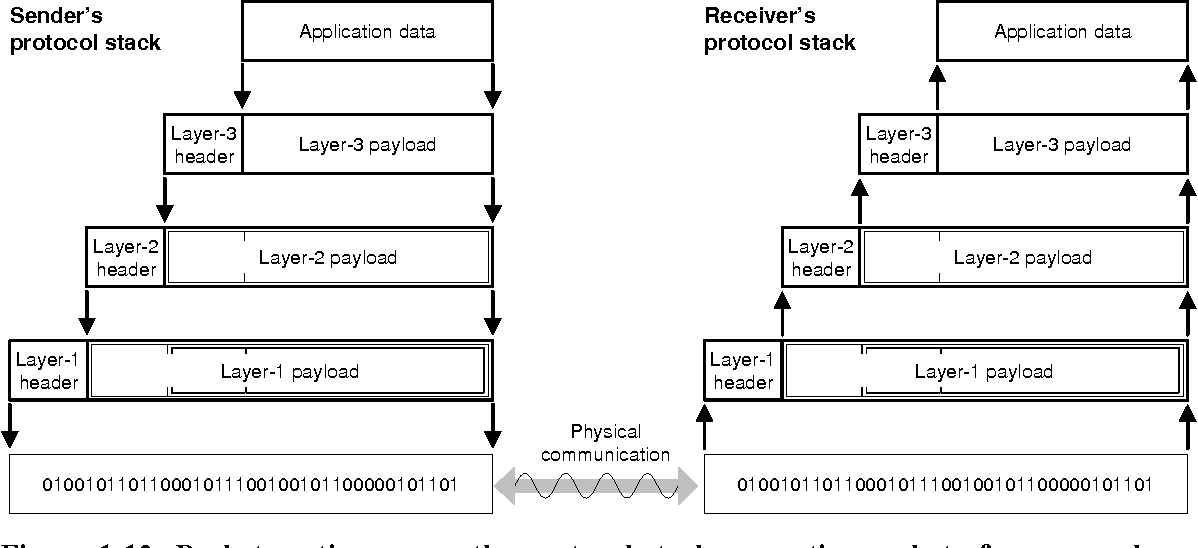
\includegraphics[width=\textwidth]{packet_layered.png}
    \caption{A Packet consists of different nested layers}%
    \label{fig:nested_layers_packet}
\end{figure}

%\subsubsection{Stacking Layers}
%The `/` operator has been used as a composition operator between two layers. When doing so, the lower layer can have one or more of its defaults fields overloaded according to the upper layer.\footnote{\url{https://scapy.readthedocs.io/en/latest/usage.html\#starting-scapy}}

 \subsubsection{Sending Packets}
 Scapy makes a distinction between sending packets at Layer-2 (L2) and Layer-3 (L3). For instance, a L3 packet is sent with the \texttt{send()}, while \texttt{sendp()} is used for L2 packets. To be able to receive answers from the network, you need to use the \texttt{sr()} and \texttt{srp()} methods. They return a tuple of two lists. The first element is a list of couples (packet sent, answer), and the second element is the list of unanswered packets. These two elements are lists, but they are wrapped by an object to present them better, and to provide them with some methods that do most frequently needed actions, e.g. \texttt{show()}.
 
 \begin{info}
     Before checking the listing below, try to understand the ICMP protocol.
 \end{info}

\begin{listing}[h]
\inputminted{python}{../code_students/example_sr.py}
\caption{Illustration of sending and receiving packets in Scapy.}%
\label{listing:example-sr}
\end{listing}

 The functions \texttt{sr1()}  and \texttt{srp1()} are variants that only return one packet that answered the packet sent. If there is no response, a \texttt{None} value will be returned when the timeout is reached. 
 
 \begin{question}
     Use wireshark to monitor the result of \texttt{ping -4 google.com} and explain. What is the purpose of the \texttt{-4} argument? 
     Use \texttt{srloop()} or \texttt{srploop()} to replicate such a ping request.\footnote{Specify the \texttt{id} field (e.g., 1), because the default value is zero and is often blocked by firewalls. } Validate the content of the DNS response in Wireshark due to pinging "google.com".
 \end{question}
 
\subsubsection{Creating packets at the Application Layer}
An example of an HTTP GET request is shown in Listings~\ref{listing:example-http-get}. It demonstrates how easy it is to include the application layer. 

\begin{listing}[h]
\inputminted{python}{../code_students/example-http-get.py}
\caption{Creating an HTTP GET request.}%
\label{listing:example-http-get}
\end{listing}



\FloatBarrier
\section{Resolve a Domain Name}
Try to complete the \textbf{DNS query} code in Listing~\ref{listing:dns-query} and change the source port to random (allowed) number.
if you are connected to a KU Leuven network, change the IP address of the DNS server to the current used DNS server by your computer because external DNS servers are blocked. The DNS server used by your computer can be found by monitoring DNS queries in Wireshark or by executing \texttt{ipconfig \textbackslash all} in your terminal.

\begin{question}
    \textbf{Explain} the choice of \textbf{variables}, e.g., which DNS type did you use and why and which source port did you use and why is it allowed to be used by user applications?
    Validate the content of the DNS response in Scapy with the DNS response shown in Wireshark.
\end{question}


\begin{listing}[h]
\inputminted[firstline=16]{python}{../code_students/dns_query.py}
\caption{DNS Query}\label{listing:dns-query}
\end{listing}

\begin{question}
    Why is the \texttt{rd} parameter specified in the DNS packet? Use \texttt{ls(DNS)} to check its default value.
\end{question}



%%%%%%%%%%%%%%%%%%%%%%%%%%%%%%%%%%%%%%%%%%%%%%%%%%%%%%%%%%%%%%%%%%%%%%%%%%%%%%%%%%%%%%%%%%
\FloatBarrier
\section{Make an ARP Request to a Friend}
\begin{question}
\begin{itemize}
    \item On which layer does ARP operate?
    \item Why is this protocol needed?
    \item What is an ARP table?
    \item What is your current ARP table and explain (what are the types)?
    \item How can you broadcast a link layer frame?
    \item Why do we need a MAC address of the other machine if we have the IP address of that machine?
\end{itemize}
\end{question}

\begin{question}
Try to resolve the MAC address of a system in your LAN\footnote{You can easily find connected systems to your local network by navigating to your default gateway or by using other services provided by your ISP, e.g., \texttt{mijn.telenet.be}. To find the IP address of your default gateway, execute  \texttt{ipconfig} in your terminal.} using the example code from Listing~\ref{listing:arp-request}.
\end{question}



\begin{listing}[h]
    \inputminted{python}{../code_students/example-arp.py}
\caption{ARP}\label{listing:arp-request}
\end{listing}

\FloatBarrier
\section{Stealth Scanning}
Stealth scanning exploits the TCP three way handshake to discover if ports are open on an Internet-accessible computer. In order to understand the working principle of this technique, study the TCP three way handshake and include this in you report.

\begin{question}
Extend the example code for the stealth attack in order to discover open ports on servers.
Try to use the \texttt{report\_ports} function of Scapy to evaluate the results of your code.
\end{question}


\begin{listing}[h]
\inputminted{python}{../code_students/stealth_scanning.py}
\caption{Stealth Scanning}%
\label{listing:stealth-scanning}
\end{listing}






% Each student writes an \textbf{individual report}. 
% This report must contain the answers to the questions and must \textbf{demonstrate} that the student has \textbf{understood} the protocols and the Scapy scripts. The following report structure is advised:
% \begin{itemize}
%     \item Title, name, year, date,\ldots
%     \item Table of contents
%     \item Introduction
%         \begin{itemize}
%             \item What?
%             \item Why?
%             \item Explain the difference between L2 and L3 communication.
%         \end{itemize}
%     \item Q\&A
%     \begin{itemize}
%         \item Make it a coherent story
%         \item Demonstrate that you understand, do not copy paste
%     \end{itemize}
%     \item Conclusion(s)\\
%     Which protocols did you investigate and what are their purpose?
%     \item References (referenced in the report)\\
%     More information regarding citing other sources can be found in this video: \url{vimeo.com/220916942}.
% \end{itemize}
% A \LaTeX\ template and tips-and-tricks can be found here: \url{github.com/dramco-edu/LaTex}. More general tips-and-tricks for writing reports can be accessed here: \url{dramco-edu.github.io/Thesis-Tips-and-Tricks/}. 

% All Python \textbf{code} must be well \textbf{documented}.
% The report and the code has to be send to \texttt{gilles.callebaut@kuleuven.be} and a printed version needs to be handed in. The \textbf{code} needs to be \textbf{included and discussed} in the \textbf{report} (no screenshots), including output (if relevant). The report can be written in Dutch or English but not both, with the exception of specific terminology. 

% \begin{description}
% 	\item[File name format]  \texttt{<firstname>\_<lastname>\_report.pdf}
% 	\item[Code name format]  \texttt{<firstname>\_<lastname>\_code.zip}
% 	\item[Language] Dutch or English (recommended)
% 	\item[Number of pages] Write your report in a compact but concise way.
% \end{description}

% %The report is expected to be structured and styled as described in~\cite{hoogenboom2012write,kallestinova2011write}.

% The deadline for handing in the report will be discussed during the lab session.
% Prior to submitting your report, check the most recent version of the assignment on \url{github.com/GillesC/Network-Capturing-and-Manipulation----Introduction-to-Wireshark-and-Scapy}.



%%%%%%%%%%%%%%%%%% Case studies %%%%%%%%%%%%%%%%%%%%%%%%%
\section{Case studies}\label{sec:use-cases}
Now that you have mastered Scapy and Wireshark, we will investigate different use cases involving network protocols. In the last three sessions, you will focus on \textbf{one} specific use case (first two sessions) and \textbf{present} your findings to your colleagues\footnote{No report is neccasary.} (last session). 

You may request a topic/use case from the list (Table~\ref{tab:use-cases}) or propose your own topic by sending a mail to \texttt{gilles.callebaut@kuleuven.be}\footnote{First come, first served applies.}. The presentation should take 10 minutes (presenting) excluding a 5 minute window for discussion and questions. Please visit \url{www.principiae.be} for excellent resources on improving your presentation skills. In this presentation, you will demonstrate what you have done. It is meant to prove that you are able to work with Scapy and Wireshark and have understood the basics of communicating on the Internet.


\begin{table}[h!]
\centering
\renewcommand{\arraystretch}{1.3}
\caption{Proposed use case (non-exhaustive list)}%
\label{tab:use-cases}
\footnotesize
%\resizebox{\textwidth}{!}{%
\begin{tabular}{@{}p{1cm} l p{4cm} p{8cm}@{}}
\toprule
Group ID &\# pers & topic & explanation \\ \midrule
1&2       & TCP reset hacking     &  This attack forces to prematurely close a TCP connection between two victim hosts. \\
2&2       & ARP spoofing       \\
3&1       & Tracerouting     & Implement tracerouting in Scapy and explain the protocol by means of examples.  \\ 
4&1 & Ping of death & Setup a PC or raspberry pi to execute a DOS ping of death attack.\\
5&2 & DNS Amplification Attack & Attack the other person by means of a DNS amplication attack. \\
6&2 & Monitoring & Capture different protocols and summarize/visualize the data over a network on a webpage. Draw conclusions based on your findings. \\
7&1 & Real-time TCP handshake & Implement the TCP handshake to be able to use upper-laying protocols such as HTTP \\
8&2 & Mitigate DOS attack (SYN flood) & Try to mitigate the SYN flood attack by inspecting the packets send by group 4.  \\
9 & 2 &pwnagotchi & Install \url{pwnagotchi.ai} and experiment with its capabilities. Show your class what you have learned and how it works.  \\
10&1& Capture a DHCP DORA & Capture the allocation and request of an IP address from the DHCP service.  \\
11&2& Build your own DNS server with a Raspberry Pi.  \\
\bottomrule
\end{tabular}%
%}
\end{table}

\FloatBarrier
\section{Evaluation}

\textbf{Small intermediate tests.}
The lab sessions will be evaluated by means of small tests at the beginning of several lab sessions. This assignment contains several questions which can help the students to assess how well they have mastered the subjects. Note that the student needs to be able to show the programming code when requested by the teaching assistant for evaluation.

\textbf{Written report (Question~4).}
In addition to the tests, Question~4 has to be executed, reported, and sent to the teaching assistant. It can be written in Dutch or English but not both, except specific terminology. 

\textbf{Presentation Use Case.}
See Section~\ref{sec:use-cases}.


\textbf{Timeline.}

Deviations from the following timeline can occur and will be communicated during the lab sessions. 

\begin{description}
    \item[Lab 1]\hfill
    \begin{itemize}
        \item Sections 1, 2 and 3 need to be fully done.
        \item Report on \textit{Q\,4}.
    \end{itemize}
    \item[Lab 2 and 3]\hfill
    \begin{itemize}
        \item Send in your report about \textit{Q\,4} before the start of lab~2.
        \item Small test about lab session 1 at the start of lab~2.
        \item Sections 4, 5 and 6 need to be fully done.
        \item Start exploring the use cases and choose a topic (first-come, first-served).
    \end{itemize}
    \item[Lab 4 and 5]\hfill
     \begin{itemize}
        \item Small test about lab sessions 2~and~3 at the beginning of lab~4.
        \item  Work on your use case.
     \end{itemize}
    \item[Lab 6]\hfill
    \begin{itemize}
        \item Present your use case.
        \item Sent all code in one \texttt{.zip} file with all code (including the questions and use case) via e-mail.
     \end{itemize}
        
\end{description}

%%%%%%%%%%%%%%%%%% APPENDIX %%%%%%%%%%%%%%%%%%%%%%%%%
\clearpage
\appendix
\section{Scapy interactive shell}\label{sec:scapy-interactive}

Scapy's interactive shell is run in a terminal session. Root privileges are needed to send the packets. However, in these lab sessions, you are primarily going to use these functions to display information concerning default values or available layers and fields.

\subsection{Entering the Scapy Environment}

The Scapy environment is accessible by executing \texttt{scapy} in a terminal:
%
\begin{lstlisting}
>scapy 
\end{lstlisting}
%
You can go out the environment with the \texttt{exit()} command.

\subsection{Available Commands}
You can check the available commands in Scapy through running \texttt{lsc()}. In the following subsections, we will discuss the commands which we will be using in these lab sessions.

\subsubsection{Help}
The \texttt{help()} function is a wrapper around pydoc.help\footnote{The pydoc module automatically generates documentation from Python modules. The documentation can be presented as pages of text on the console, served to a Web browser, or saved to HTML files} that provides a helpful message when `help' is typed at the Python interactive prompt.

\begin{itemize}
  \item Calling \texttt{help()} at the Python prompt starts an interactive help session.
  \item Calling \texttt{help(thing)} prints help for the python object `thing'.
\end{itemize}

\subsubsection{List Available Protocols}
You can list the available protocols and fields for each layer by using \texttt{ls()}. 
If you run this command without an argument, all the supported protocols are listed.
When including a protocol as the argument, e.g. \texttt{ls(ARP)}, the fields and their defaults will be displayed.

%\subsubsection{show\_interfaces()}


\end{document}
